\documentclass{beamer}

\usetheme[progressbar=frametitle]{metropolis}
\usepackage{appendixnumberbeamer}
\usepackage{booktabs}
\usepackage{amsmath}
\usepackage{amssymb}
\usepackage{tcolorbox}
\usepackage{adjustbox}
\usepackage{graphicx}
\usepackage{caption}
\usepackage{hyperref}
\definecolor{metropolisblue}{RGB}{39, 59, 94}
\setbeamersize{text margin left=0.5cm,text margin right=1cm}
\captionsetup[figure]{labelformat=empty}
\newcommand{\data}{\mathcal{D}}
\newenvironment{myitemize}{%
\begingroup
    \setbeamercolor{itemize item}{parent=structure}
    \setbeamercolor{alerted text}{fg=black}
    \setbeamercolor{itemize/enumerate body}{fg=white}
    \begin{itemize}[<alert@+->]
}{
    \end{itemize}
\endgroup
}
\hypersetup{
    colorlinks=true,
    linkcolor=blue,
    urlcolor=blue
}

% Begin document
\begin{document}

% Title page
\title{Laplace Approximation}
\author{Zeel B Patel, Nipun Batra}
\date{\today}
\institute{IIT Gandhinagar}
\maketitle


\begin{frame}{Outline}
    \begin{columns}
        \begin{column}{0.5\textwidth}
            \tableofcontents
        \end{column}
        \begin{column}{0.5\textwidth}
            % add two subfigures from top to bottom
            \begin{figure}
                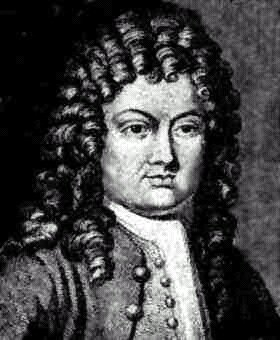
\includegraphics[width=0.4\textwidth]{../figures/laplace-approx/Taylor.jpg}
                \caption*{Brook Taylor}
            \end{figure}
            \begin{figure}
                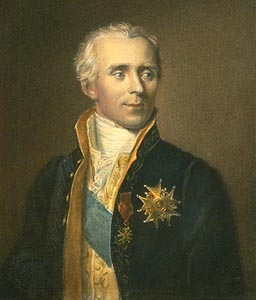
\includegraphics[width=0.4\textwidth]{../figures/laplace-approx/Laplace.jpg}
                \caption*{Pierre-Simon Laplace}
            \end{figure}

        \end{column}
    \end{columns}
\end{frame}

\begin{frame}{Overall idea}
    \begin{itemize}
        \item Posterior distribution $p(\boldsymbol{\theta}| \mathcal{D})$ might be intractable but we can compute the MAP estimate.
        \item We know that posterior would be in form: $p(\boldsymbol{\theta}| \mathcal{D}) = \frac{1}{Z}p(\mathcal{D}, \boldsymbol{\theta})$, where $Z$ is the normalizing constant.
        \item We can approximate this posterior using Taylor series expansion around the MAP estimate and it turns out that, after making a few assumptions, the resulting distribution is a Gaussian: $p(\boldsymbol{\theta}| \mathcal{D}) \approx \mathcal{N}(\boldsymbol{\theta}|\boldsymbol{\theta}_{MAP}, H^{-1})$, where $H$ is the Hessian matrix of the log joint evaluated at $\boldsymbol{\theta}_{MAP}$.
    \end{itemize}
\end{frame}

\section{Taylor Series Expansion}

\begin{frame}{1D Taylor Series}
    \begin{equation*}
        \tilde{f}(x) = f(x_0) + f'(x_0)(x-x_0) + \frac{f''(x_0)}{2!}(x-x_0)^2 + \frac{f'''(x_0)}{3!}(x-x_0)^3 + \dots
    \end{equation*}

\end{frame}

\begin{frame}{Taylor Approximation of a 1D Function}
    Consider the following function:
    \begin{equation*}
        f(x) = \sin(1+x)
    \end{equation*}
    \begin{figure}
        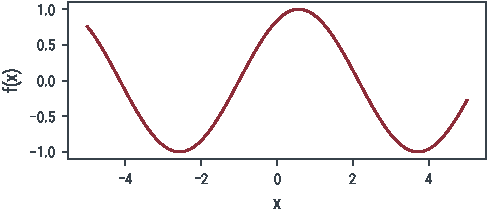
\includegraphics[width=0.8\textwidth]{../figures/laplace-approx/sin.pdf}
    \end{figure}

\end{frame}

\newcommand{\taylor}[1]{
    \begin{frame}{Taylor Approximation of a 1D Function}
        Taylor approximation at $x_0 = 0$:
        \begin{figure}
            \includegraphics[width=0.8\textwidth]{../figures/laplace-approx/sin-taylor-#1.pdf}
        \end{figure}
    \end{frame}
}

\taylor{0}
\taylor{1}
\taylor{2}
\taylor{3}
\taylor{4}
\taylor{5}
\taylor{12}

\begin{frame}{Taylor Approximation of a 1D Gaussian Function}
    Consider the standard normal distribution: $p(x) \sim \mathcal{N}(x|0, 1)$\\
    \begin{equation*}
        p(x) = \frac{1}{\sqrt{2\pi}}e^{-\frac{x^2}{2}}
    \end{equation*}

    \begin{figure}
        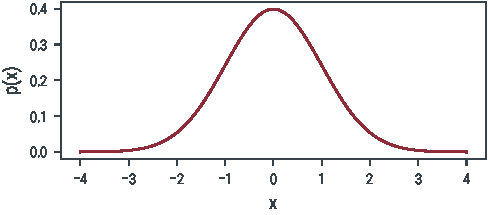
\includegraphics[width=0.8\textwidth]{../figures/laplace-approx/standard-normal.pdf}
    \end{figure}

\end{frame}

\begin{frame}{Taylor Approximation of a 1D Gaussian Function}
    We will try to approximate log of the above function using Taylor series expansion around $x_0 = 0$.\\
    \pause
    \begin{align*}
        \onslide<2->{f(x)                      & = \log p(x) = \log \left(\frac{1}{\sqrt{2\pi}}\right) - \frac{x^2}{2}} \\
        \onslide<3->{f(0)                      & = \log \left(\frac{1}{\sqrt{2\pi}}\right)}                             \\
        \onslide<4->{f'(0)\cdot x              & = -x_0 \cdot x = 0}                                                    \\
        \onslide<5->{f''(0)\cdot \frac{x^2}{2} & = -1 \cdot \frac{x^2}{2}}
    \end{align*}
    \begin{equation*}
        \onslide<6->\text{Taylor approximated } \tilde{f}(x) = \log \left(\frac{1}{\sqrt{2\pi}}\right) - \frac{x^2}{2}
    \end{equation*}

\end{frame}

\section{ND Taylor Series}

\begin{frame}{ND Taylor Series}
    \begin{equation*}
        \tilde{f}(\boldsymbol{x}) = f(\boldsymbol{x}_0) + \nabla f(\boldsymbol{x}_0)^T(\boldsymbol{x}-\boldsymbol{x}_0) + \frac{1}{2}(\boldsymbol{x}-\boldsymbol{x}_0)^T \nabla^2 f(\boldsymbol{x}_0)(\boldsymbol{x}-\boldsymbol{x}_0) + \dots
    \end{equation*}
\end{frame}

\begin{frame}{Approximate a 2d function}
    We take the following function:
    \begin{equation*}
        f(x_1, x_2) = \sin(1 + x_1 + x_2)
    \end{equation*}

    \begin{figure}
        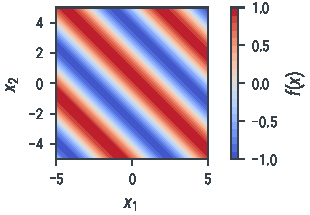
\includegraphics[]{../figures/laplace-approx/sin2d.pdf}
    \end{figure}

\end{frame}

\begin{frame}{Approximate a 2d function}
    Taylor approximation at $x_0 = (0, 0)$:
    \begin{figure}
        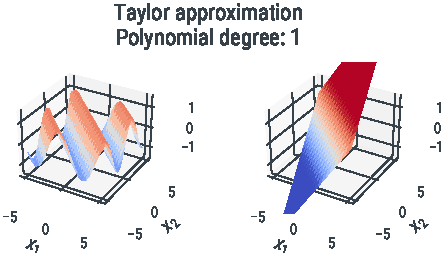
\includegraphics[width=0.6\textwidth]{../figures/laplace-approx/sin2d-taylor-1.pdf}
    \end{figure}
    \begin{figure}
        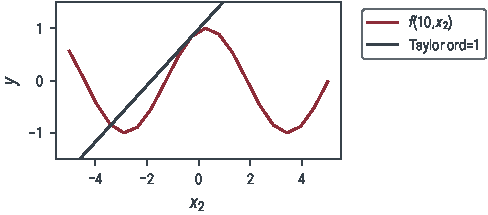
\includegraphics[width=0.6\textwidth]{../figures/laplace-approx/sin2d-taylor-1d-1.pdf}
    \end{figure}

\end{frame}

\begin{frame}{Approximate a 2d function}
    Taylor approximation at $x_0 = (0, 0)$:
    \begin{figure}
        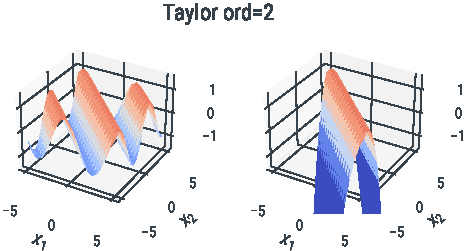
\includegraphics[width=0.6\textwidth]{../figures/laplace-approx/sin2d-taylor-2.pdf}
    \end{figure}
    \begin{figure}
        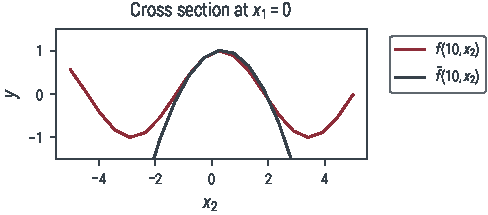
\includegraphics[width=0.6\textwidth]{../figures/laplace-approx/sin2d-taylor-1d-2.pdf}
    \end{figure}

\end{frame}

\section{Laplace Approximation}

\begin{frame}{Laplace Approximation}
    \begin{equation*}
        p(\boldsymbol{\theta}| \mathcal{D}) = \frac{1}{Z}p(\mathcal{D}, \boldsymbol{\theta})
    \end{equation*}
    \pause
    We can rewrite this as:
    \begin{align*}
        p(\boldsymbol{\theta}| \mathcal{D}) & = \frac{1}{Z}e^{-f(\boldsymbol{\theta)}}    \\
        f(\boldsymbol{\theta})              & = -\log p(\mathcal{D}, \boldsymbol{\theta})
    \end{align*}
    \pause
    Note that $f(\boldsymbol{\theta})$ is the negative log joint which is used as a loss function to estimate $\boldsymbol{\theta}_{MAP}$.
\end{frame}

\begin{frame}{Laplace Approximation}
    \begin{itemize}
        \item Highest mass is concentrated around $\boldsymbol{\theta}_{MAP}$ and hence it makes sense to get Taylor approximation around that point.
              \pause
        \item In other words, if our approximation is bad where we have low probability mass, it doesn't matter much.
              \pause
        \item Thus, we approximate $f(\boldsymbol{\theta})$ as $\tilde{f}(\boldsymbol{\theta})$ around $\boldsymbol{\theta}_{MAP}$ using Taylor series expansion up to second derivative:
    \end{itemize}
    \begin{align*}
        \tilde{f}(\boldsymbol{\theta}) & = f(\boldsymbol{\theta}_{MAP}) + \nabla f(\boldsymbol{\theta}_{MAP})^T(\boldsymbol{\theta}-\boldsymbol{\theta}_{MAP})                                     \\
                                       & \quad + \frac{1}{2}(\boldsymbol{\theta}-\boldsymbol{\theta}_{MAP})^T \nabla^2 f(\boldsymbol{\theta}_{MAP})(\boldsymbol{\theta}-\boldsymbol{\theta}_{MAP})
    \end{align*}
\end{frame}


\begin{frame}{Laplace Approximation}
    \begin{align*}
        \onslide<1->{\tilde{f}(\boldsymbol{\theta}) & = f(\boldsymbol{\theta}_{MAP}) + \nabla f(\boldsymbol{\theta}_{MAP})^T(\boldsymbol{\theta}-\boldsymbol{\theta}_{MAP})                                      \\
                                                    & \quad + \frac{1}{2}(\boldsymbol{\theta}-\boldsymbol{\theta}_{MAP})^T \nabla^2 f(\boldsymbol{\theta}_{MAP})(\boldsymbol{\theta}-\boldsymbol{\theta}_{MAP})}
    \end{align*}
    \onslide<2->{Since, $\boldsymbol{\theta}_{MAP}$ is minima of $f(\boldsymbol{\theta})$, $\nabla f(\boldsymbol{\theta}_{MAP}) = 0$.}

    \begin{align*}
        \onslide<3->{\tilde{f}(\boldsymbol{\theta}) & = f(\boldsymbol{\theta}_{MAP}) + \frac{1}{2}(\boldsymbol{\theta}-\boldsymbol{\theta}_{MAP})^T \nabla^2 f(\boldsymbol{\theta}_{MAP})(\boldsymbol{\theta}-\boldsymbol{\theta}_{MAP})} \\
        % \onslide<4->{                       & = f(\boldsymbol{\theta}_{MAP}) + \frac{1}{2}(\boldsymbol{\theta}-\boldsymbol{\theta}_{MAP})^T H(\boldsymbol{\theta}-\boldsymbol{\theta}_{MAP})}
    \end{align*}
    \onslide<4->{where $\nabla^2 f(\boldsymbol{\theta}_{MAP})$ is the Hessian matrix of $f(\boldsymbol{\theta})$ evaluated at $\boldsymbol{\theta}_{MAP}$.}

\end{frame}

\begin{frame}{Laplace Approximation}
    Plugging this back to the posterior equation:

    \begin{align*}
        \onslide<1->{p(\boldsymbol{\theta}| \mathcal{D}) & = \frac{1}{Z}e^{-f(\boldsymbol{\theta)}} \;\;\;\;\; \text{where } f(\boldsymbol{\theta}) = -\log p(\mathcal{D}, \boldsymbol{\theta})
        }                                                                                                                                                                                                                                                                \\
        \onslide<2->{                                    & \approx \frac{1}{Z}e^{-f(\boldsymbol{\theta}_{MAP})}e^{-\frac{1}{2}(\boldsymbol{\theta}-\boldsymbol{\theta}_{MAP})^T \nabla^2 f(\boldsymbol{\theta}_{MAP})(\boldsymbol{\theta}-\boldsymbol{\theta}_{MAP})}}   \\
        \onslide<3->{                                    & = \frac{1}{Z}p(\mathcal{D}, \boldsymbol{\theta}_{MAP})e^{-\frac{1}{2}(\boldsymbol{\theta}-\boldsymbol{\theta}_{MAP})^T \nabla^2 f(\boldsymbol{\theta}_{MAP})(\boldsymbol{\theta}-\boldsymbol{\theta}_{MAP})}}
        % \onslide<5->{Z                                   & = p(\mathcal{D}, \boldsymbol{\theta}_{MAP}) \cdot (2\pi)^{D/2} \cdot |\nabla^2 f(\boldsymbol{\theta}_{MAP})|^{-\frac{1}{2}}}
    \end{align*}
    \onslide<4->{
        \begin{tcolorbox}
            \begin{align*}
                p(\boldsymbol{\theta}| \mathcal{D}) & \approx \mathcal{N}\left(\boldsymbol{\theta}|\boldsymbol{\theta}_{MAP}, \left(\nabla^2 f(\boldsymbol{\theta}_{MAP})\right)^{-1}\right) \\
                Z                                   & = p(\mathcal{D}, \boldsymbol{\theta}_{MAP}) \cdot (2\pi)^{D/2} \cdot |\nabla^2 f(\boldsymbol{\theta}_{MAP})|^{-\frac{1}{2}}
            \end{align*}
        \end{tcolorbox}
    }
    % \onslide<5->{Note that this result is not specific to Bayesian inference and can be used to approximate any intractable function.}

\end{frame}

\begin{frame}{Pros and Cons of Laplace Approximation}
    \begin{itemize}
        \item Pros:
              \begin{itemize}
                  \item Simple to implement
                  \item Computationally efficient
                  \item Can be used to approximate any intractable function
              \end{itemize}
              \pause
        \item Cons:
              \begin{itemize}
                  \item It can give bad approximation when posterior is not unimodal
                  \item Gaussian assumption can be too restrictive at times
                  \item Hessian matrix inversion can be numerically unstable and expensive. A diagonal or block-wise approximation can be applied to resolve this. Checkout \href{https://github.com/AlexImmer/Laplace}{Laplace-Redux} for more details.
              \end{itemize}
    \end{itemize}

\end{frame}

\begin{frame}{Beta-Bernoulli Coin Toss}
    Let's take Beta-Bernoulli Coin Toss example since we know the closed form posterior for it. Consider the following scenario:
    \pause
    \begin{itemize}
        \item $\mathcal{D} = \{1, 1, 1, 1, 1, 1, 1, 1, 0\}$
        \item $p(\theta) = \text{Beta}(\alpha=2, \beta=2)$
        \item $h = \theta$
        \item $p(y|h) = h^y(1-h)^{1-y}$
    \end{itemize}
    \pause
    \begin{figure}
        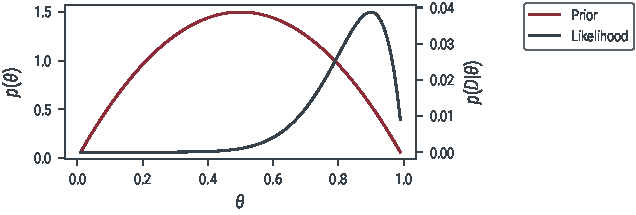
\includegraphics[]{../figures/laplace-approx/beta-prior-coin-toss.pdf}
    \end{figure}
\end{frame}

\begin{frame}{Beta-Bernoulli Coin Toss}
    MAP estimate:
    \begin{figure}
        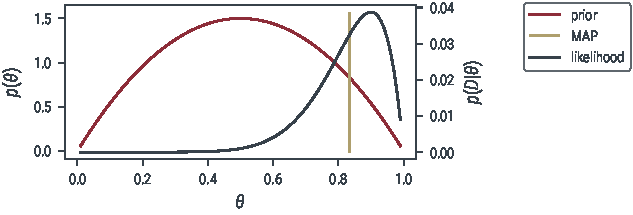
\includegraphics[]{../figures/laplace-approx/beta-prior-coin-toss-map.pdf}
    \end{figure}
\end{frame}

\begin{frame}{Beta-Bernoulli Coin Toss}
    Laplace Approximation:
    \begin{figure}
        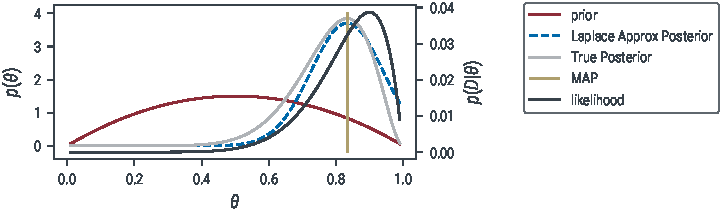
\includegraphics[]{../figures/laplace-approx/beta-prior-coin-toss-laplace.pdf}
    \end{figure}
\end{frame}

\begin{frame}{Normal Prior for Coin Toss}
    Consider the following coin toss experiment scenario:
    \begin{itemize}
        \item $\mathcal{D} = \{1, 1, 1, 1, 1, 1, 1, 1, 0\}$
        \item $p(\theta) = \mathcal{N}(\theta|\mu=-2, \sigma=1)$
        \item $h = \sigma(\theta)$
        \item $p(y|\theta) = h^y(1-h)^{1-y}$
    \end{itemize}
    \begin{figure}
        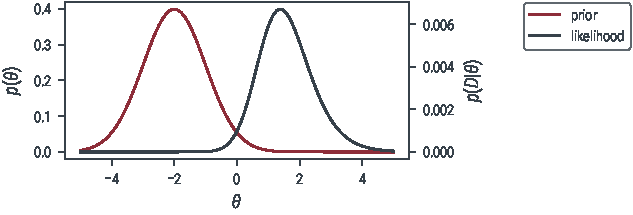
\includegraphics[]{../figures/laplace-approx/normal-prior-coin-toss.pdf}
    \end{figure}
\end{frame}

\begin{frame}{Normal Prior for Coin Toss}
    First, we find the MAP estimate.
    \begin{figure}
        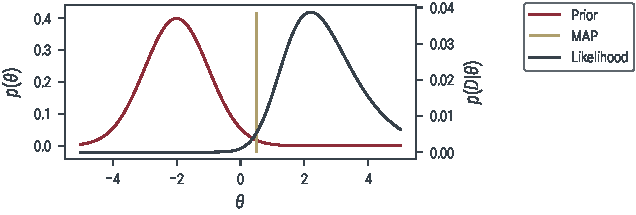
\includegraphics[]{../figures/laplace-approx/normal-prior-coin-toss-map.pdf}
    \end{figure}
\end{frame}

\begin{frame}{Normal Prior for Coin Toss}
    Now, according to the Laplace Approximation, the posterior is:
    \begin{figure}
        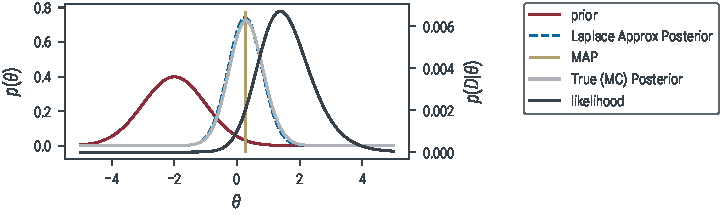
\includegraphics[]{../figures/laplace-approx/normal-prior-coin-toss-laplace.pdf}
    \end{figure}
    We got True (MC) Posterior by a Monte Carlo estimation of the evidence.
\end{frame}

\begin{frame}{Multi-Mode example}
    Consider a Gaussian Mixture distribution with two modes. We assume that, it is an unnormalized density and we want to get normalized Laplace approximation of it.
    \pause
    \begin{equation*}
        p(\theta) = \frac{7}{10}\mathcal{N}(\theta|-2, 1) + \frac{3}{10}\mathcal{N}(\theta|2, 1)
    \end{equation*}
    \pause
    \begin{figure}
        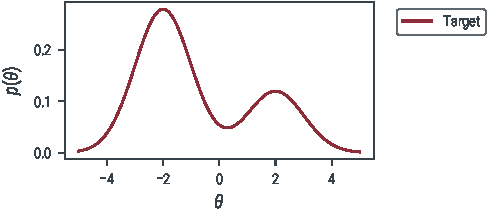
\includegraphics[]{../figures/laplace-approx/mixture-density.pdf}
    \end{figure}

\end{frame}

\begin{frame}{Multi-Mode example}
    Laplace Approximation:
    \begin{figure}
        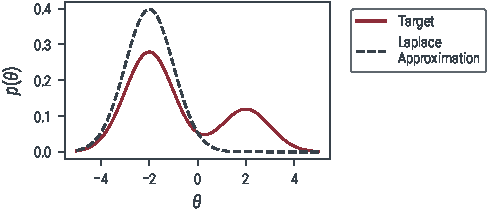
\includegraphics[]{../figures/laplace-approx/mixture-density-laplace.pdf}
    \end{figure}
\end{frame}

\end{document}